\section{Grundlagen}
\label{sec:grundlagen}

In dieser Seminararbeit werden verschiedene Technologien verwendet die für die Anwendung im Cloud und Edge Robotics Bereich relevant sind. Darunter befinden sich breitere Themenbereiche wie die Cloud oder das Edge Computing. Es werden aber auch speziellere Technologien wie ROS2 oder Zenoh für die Nutzung mit Robotern oder zur Kommunikation betrachtet. In diesem Abschnitt werden die Grundbegriffe und Technologien rund um das Cloud und Edge Robotics vorgestellt und im Kontext erläutert.

\subsection{Cloud-To-Thing Kontinuum} % (fold)
\label{sub:Cloud-To-Thing-Continuum}

Das \acrlong{cttc} beschreibt die Möglichkeit zur Nutzung von Speicher und Rechenkapazitäten, sowie der Sammlung von Daten auf einem Kontinuum. Das Kontinuum enthält, wie in \cite{cominardiDevopsEdgeopsVision2021} beschrieben, verschiedene Arten von Ressourcen die sich in mehreren Netzwerken oder geographischen Orten befinden. Die Ressourcen reichen von Roboter, über Edge Server bis hin zu Cloud Instanzen.

\begin{figure}
  \begin{center}
    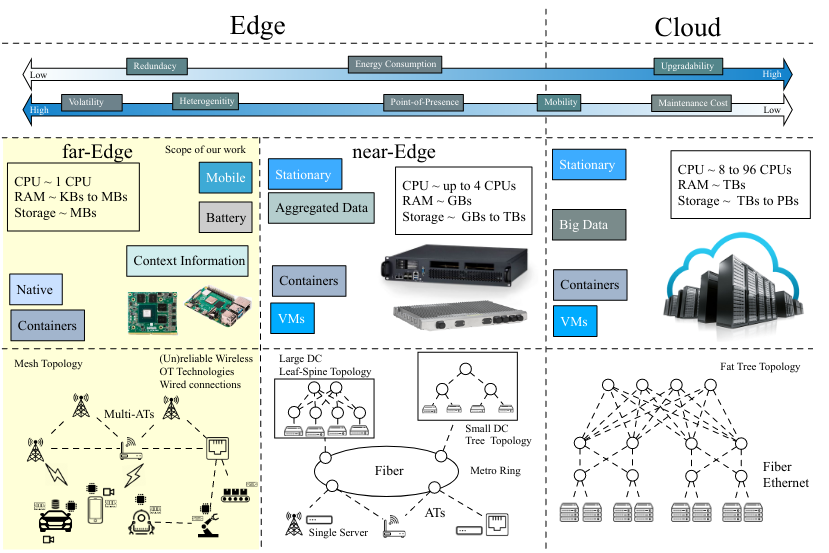
\includegraphics[width=0.95\textwidth]{./figures/cloud-thing-continuum.png}
  \end{center}
  \caption{Übersicht \acrlong{cttc} \cite{baldoniManagingFarEdgeAre2021}}
  \label{fig:cttc}
\end{figure}

Wie man in der Grafik \ref{fig:cttc} erkennen kann, hat man unterschiedliche heterogene Ressourcen die verschiedene Eigenschaften haben und unter verschiedenen Bedingungen agieren. Auf der einen Seite, hat man am Edge ein sehr heterogenes System mit Beispielsweise Robotern und IoT Geräten. Diese besitzen eingeschränkte Ressourcen wie Beispielsweise Rechenkapazitäten. Hinzu kommen unverlässliche Verbindungen wie Wi-Fi oder Bluetooth.\\
Auf der anderen Seite, befinden sich die Cloud Instanzen. Dessen Ressourcen sind recht homogen und verlässlich. Größtenteils also das genaue Gegenteil zu den Geräten nahe dem Edge. Zwischen den beiden Schichten befinden sich oftmals Edge Server. Diese ähneln den Komponenten der Cloud. Da sie aber von der Lokalität nahe an den Endgeräten sein müssen, sind Sie nicht so einfach Skalierbar wie Cloud Ressourcen.\\
Aufgrund der unterschiedlichen Gegebenheiten und Eigenschaften der Geräte, ist es wichtig ein einheitliches Kommunikationsmedium zu nutzen welches die Komponenten der verschiedenen Schichten unterstützt. Im Bereich der Robotik, wurden diese Aspekte ende 2018 in \cite{jawharNetworkingMultiRobotSystems2018} untersucht. Im Artikel wurde das \acrlong{cttc} als R2I(robot-to-infrastructure) beschrieben. Dabei wurden MRS(Multi-Robot-Systems) und die Möglichkeiten der Kommunikation verglichen. Beim Vergleich kamen die Autoren zu einer Ähnlichen Schlussfolgerung wie eingangs erwähnt: "This gateway node must be able to map the networking parameters associated with the data traffic in the data link layer header to the corresponding data link layer header in the infrastructure network." \cite{jawharNetworkingMultiRobotSystems2018}. Gemeint, sind die verschiedenen Protokolle die unterstützt werden müssen um sowohl Robotik als auch weitere Infrastruktur Systeme miteinander zu verbinden. Das Paper beschreibt zudem Grundprotokolle wie Wi-Fi oder Bluetooth die zum Austausch der Nachrichten benötigt werden. Wie man an den zahlreichen im Paper genannten Technologien erkennen kann, ist der Bereich um die Kommunikation im Robot to Infrastructure Bereich sehr Komplex. Das \acrlong{cttc} zielt dabei auf eine Vereinheitlichung der Kommunikationswege aus. Dabei wird eine Technologie gesucht, die bereits bestehende Protokolle unterstützt, abstrahiert oder ersetzt und als Ende zu Ende Lösung genutzt werden kann. Im folgenden Teil dieser Arbeit wird sich dieser Frage gewidmet.


\subsection{Edge Computing}

Das Ziel hinter Edge Computing ist es zum einen, Rechen oder Speicher Ressourcen näher an die Clients zu bringen. Edge Computing Server dienen dabei als Schnittstelle zwischen IoT Geräten und Datenzentren die sich in der Cloud befinden können \cite{luntovskyyHighlyDistributedSystemsIoT2022}.\\
Das Konzept wurde im modernen Kontext erstmals 2012 in einem Paper von dem Unternehmen Cisco vorgestellt \cite{bonomiFogComputingIts}. Dabei wurde es als Erweiterung der Cloud zur Unterstützung von Internet of Things (IoT) Anwendungen definiert. Anzumerken sei, dass im Paper der Begriff 'Fog' für 'Edge' genutzt wird. Beide werden in der Literatur oftmals als Synonym genutzt. In dieser Arbeit, wird der Begriff 'Edge' eingesetzt.\\
Wie also beschrieben, ist das Edge Computing eine besondere Art der Bereitstellung von Ressourcen für Clients. Aus diesem Grund, kann man mehrere Eigenschaften ausmachen die für das Edge computing von Bedeutung sind\cite{bonomiFogComputingIts}:

\begin{enumerate}
  \item Standorts Bewusstsein und geringe Latenz: Edge Knoten werden vornehmlich in der Näher von Clients plaziert. Dadurch können diese entlastet werden ohne dass es zu großen Latenz Problemen kommt.
    \item Geografische Verteilung: Um die nähe der Clients zu gewährleisten, werden die Edge Knoten an verschiedenen Orten angebracht. Dies muss beim Deployment der Knoten beachtet werden.
      \item Beweglichkeit: Im gegensatz zu stationäre Server, sind Edge Instanzen in Ihrem Ort beweglich. Dies ist nötig um Clients an unterschiedlichen Orten zu unterstützen und flexibel zu bleiben. Dafür wird ein System gebraucht welches den jeweiligen Edge Host von seinem Ort entkoppelt und Änderungen am Standort wahrnimmt und unterstützt.
        \item Echtzeit Kommunikation: Edge Knoten müssen in Echtzeit mit Endanwendungen kommunizieren können. Eine Verarbeitung in Form von zum Beispiel eine Warteschlange ist hier nicht möglich, da Clients auf die Antwort des Edge Servers womöglich angewiesen sind.
\end{enumerate}

Edge Computing unterscheidet sich dabei in verschiedenen Aspekten vom regulären Cloud Computing. Verbindungen haben in diesem Kontext oftmals eine viel größere Lebensspanne. Das heißt, dass die Verbindungen nicht wie bei regulären Internetdiensten nach einer kurzen Zeit wieder geschlossen werden. Ebenfalls, gibt es im Bereich des Edge Computings sehr viele heterogene Clients. Im Kontext der Robotik, könnte man zum Beispiel Verbindungen von einem mobilen Roboter und einem stationären Greifarm unterscheiden. Besonders eindrucksvoll ist dies im IoT Bereich, in dem man sehr viele verschiedene Verbindungen verarbeiten muss.\\
Diese Eigenschaften haben verschiedene Vorteile gegenüber dem regulären Cloud Computing. Einerseits, kann eine kürzere Distanz zum Server die Latenz der Verbindungen verbessern. Andererseits, kann es zu einer direkten Datenannahme und Pre-Prozessierung der Daten direkt am Standort kommen. Dies ist hilfreich, wenn die Datenverarbeitung für die Funktionalität des Roboters von Relevanz ist \cite{luntovskyyHighlyDistributedSystemsIoT2022}.

\begin{figure}
  \centering
  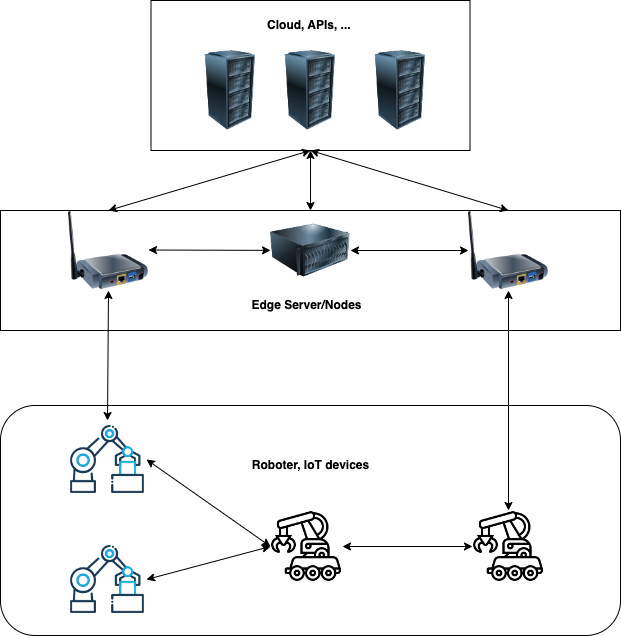
\includegraphics[width=0.5\textwidth]{./figures/edge-computing.png}
  \caption{Vereinfachte Edge Computing Architektur}
  \label{fig:edge-computing}
\end{figure}

Trotz der Allgegenwärtigkeit von Cloud Computing Services in unserem Alltag\cite{GartnerForecastsWorldwide2022}, gibt es im Edge Computing Bereich noch einige Herausforderungen. Eine davon ist die Konnektivität zwischen den Edge Knoten und den jeweiligen Geräten wie beispielsweise den Robotern. Das Wunschszenario wären hier hohe Datenraten mit möglichst niedrigen Verbindungsverzögerungen \cite{groshevEdgeRoboticsAre2022}. Dies ist aber oftmals durch äußere Einflüsse nicht reibungslos möglich. Beispielsweise spielt die Standort Wahrnehmung hier eine Rolle. Ein Roboter, der sich näher am Edge Knoten befindet kann auch von einer besseren Konnektivität profitieren.

Ziel ist es also die Zusammenarbeit zwischen Heterogene Ressourcen wie beispielsweise Roboter und Edge Knoten zu verbessern. Dafür müssen verschiedene Variablen berücksichtigt werden. Unter anderem die Konnektivität, die geographische Verteilung der Knoten oder der spezielle Use Case der umgesetzt werden soll.\\
In \ref{fig:edge-computing} ist eine vereinfachte Edge Architektur dargestellt. Hier hat man in der untersten Schicht mehrere Roboter die Dienste von einer Edge Instanz nutzen. Die Edge Instanzen können sich dabei direkt bei den Robotern befinden (Bspw. in einer Fabrik) oder nur geographisch an einem nähern Ort als Cloud Server. Durch die nähere Distanz ist aus performance Sicht eine Auslagerung überhaupt möglich. In der obersten Schicht, sind die für Roboter Betriebs irrelevante Services angesiedelt. Diese können zum Beispiel Cloud Schnittstellen sein, die Berechnungen anhand der gesammelten Daten an der Edge ausführen.


\subsection{Cloud Computing}

Cloud Computing ist ein sehr großer und weitreichender Begriff der in den letzten Jahren sehr stark gewachsen ist. Rimal et al. \cite{rimalArchitecturalRequirementsCloud2011} beschreibt Cloud Computing folgendermaßen: "Cloud Computing is a model of service delivery and access where dynamically scalable and virtualized resources are provided as a service over the Internet.". Wie in der Definition erwähnt, bietet Cloud computing einen großen Vorteil gegenüber traditionellen, selbst betriebene Servern. Bei Cloud Computing hat man dabei zum einen die Möglichkeit Ressourcen nahezu beliebig zu nutzen und nach Bedarf Skalieren. Zum anderen bietet Cloud Computing nicht nur Zugang zu reiner Rechenleistung oder Speicherplatz, sondern auch zu spezialisierten Services wie Machine Learning spezifische Anwendungen oder Big Data Lösungen\cite{antonopoulosCloudComputingPrinciples2017}.\\

Cloud Computing Services lassen sich in drei verschiedene Modele einteilen \cite{antonopoulosCloudComputingPrinciples2017}:

\begin{enumerate}
  \item Infrastructure as a Service (IaaS): IaaS ist die grundlegendste Art Ressourcen aus der Cloud zu beziehen. Dabei bezieht man Ressourcen wie Rechen oder Speicherleistung direkt über das Internet und kann darüber verfügen. Ein Vorteil von Infrastructure as a Service ist, dass es möglich ist nur für die genutzten Ressourcen zu zahlen.
  \item Platform as a Service (PaaS): PaaS befindet sich eine Stufe über dem IaaS und bietet Nutzern eine Platform an die all jene Systeme schon enthält die man für den jeweiligen Use Case braucht. Beim Platform as a Service, muss man sich keine Gedanken über die Planung von Ressourcen oder das aufsetzen von Systemen machen. Dies wird alles von dem jeweiligen Anbieter übernommen und spart dem Endanwender sowohl Zeit als auch know how über die darunterliegenden Systemen.
  \item Software as a Service (SaaS): SaaS ist die höchste Stufe des Cloud Computing und bietet dem Nutzer fertige Softwarelösungen an. Eine Besonderheit hier ist, dass ich viele verschiedene Nutzer die Ressourcen einer Anwendung teilen die sie gemeinsam nutzen. Anwender haben hier den leichtesten Zugang zu einer bestimmten Lösung, jedoch die kleinste individuelle Anpassbarkeit.
\end{enumerate}

Neben den Arten der Cloud Services, gibt es ebenfalls verschiedene Modelle und Cloud Lösungen bereitzustellen \cite{antonopoulosCloudComputingPrinciples2017}:

\begin{enumerate}
  \item Public Cloud: Dies ist die populärste Art Cloud Lösungen einzusetzen und richtet sich an die Allgemeinheit der Nutzer. Cloud Computing Ressourcen sind dabei für jeden über öffentliche Anbieter verfügbar und können je nach Bedarf skaliert werden.
  \item Private Cloud: Das Model der Privaten Cloud wird meistens von Unternehmen und Organisationen genutzt. Dabei werden Ressourcen und Netzwerkzugänge von der jeweiligen Institution selbst verwaltet. Private Cloud Modelle haben Vorteile, wenn die Sicherheit und Gesetzliche Vorgaben hohe Priorität haben. Das Hosting, wird bei Private Cloud Modelle oft durch die die Nutzer selber betrieben.
  \item Hybrid Cloud: Wie der Name schon verrät, handelt es sich hierbei um eine Kombination aus öffentlichen und privater Cloud. Diese können kombiniert werden, um sicherheitsrelevante von allgemein zugänglichen Services zu trennen.
\end{enumerate}

Die im Cloud Computing angebotenen Eigenschaften sind dabei sehr hilfreich für die Robotik. Vor allem spielt die Rechenintensive Auswertung der Daten eine wichtige Rolle. Roboter können dabei gesammelte Informationen direkt an Servern in der Cloud schicken die diese auf verschieden Arten auswerten können oder für die weitere Verarbeitung zwischenspeichern können. Weitere Anwendungen und dahingehende Details werden im Laufe dieser Arbeit behandelt.


\subsection{Robotik Systeme} % (fold)
\label{sub:Robotik Systeme}

Roboter kommen immer mehr in Bereichen der Industrie und Haushalt zum Einsatz. Dafür essentiell ist ein System, welches Abstraktionen für die Roboter Systeme bereitstellt und die Konnektivität zwischen den Roboter Schnittstellen herstellt. Eine wichtige Voraussetzung für ein möglicher Standard ist die Unterstützung möglichst vieler Systeme. Die Bandbreite unterschiedlicher Systemen ist mit einfachen embedded Systemen, Industrie Roboter oder Systeme für Selbstfahrende Fahrzeuge sehr Breitgefächert.\\
Mit dem \acrlong{ros} (ROS) der Open Source Robotics Foundation (OSRF) wurde dabei ein System entwickelt, welches die oberen Voraussetzungen erfüllt und sich unter den Robotik Systemen als Standard etabliert hat. Im folgenden wird ROS und die dessen weiterentwicklung ROS 2 vorgestellt. Da im Kontext dieser Arbeit die Kommunikation zwischen Cloud, Edge und Robotik Systemen im Vordergrund steht, werden ebenfalls die Protokolle betrachtet die den Austausch zwischen den verschiedenen Systemen unter sich ermöglichen.

\subsubsection{ROS 2} % (fold)
\label{ssub:ROS 2}

ROS \cite{ConceptsROSDocumentation} ist ein Betriebssystem das verschiedene Arten von Robotern unterstützt. ROS2 ist dabei die zweite Version des Betriebssystems und bringt zahlreiche Änderungen im Aufbau der Komponenten mit sich. Es bietet verschiedene Abstraktionen von Sensoren oder Entwicklungswerkzeige mit sich die wichtig bei der Arbeit im Robotik Bereich sind.\\
ROS hatte zahlreiche Nachteile die als Motivation für die Entwicklung von ROS2 dienten \cite{maruyamaExploringPerformanceROS22016}. Zum einen läuft ROS nur auf Linux und verbraucht viele Ressourcen. Zum anderen und viel wichtiger jedoch, unterstützt es keine Echtzeit Anwendungen \cite{ConceptsROSDocumentation}. Dazu kommt die schlechte Fehlertoleranz und Prozess Synchronisation.\\
ROS2 verbessert die oben genannten Aspekte in dem es eine vollkommen neue Architektur einführt.

\begin{figure}
  \centering
  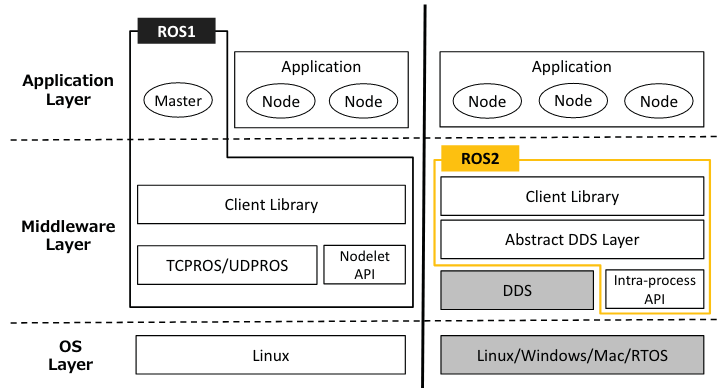
\includegraphics[width=0.95\textwidth]{./figures/ros2-architecture.png}
  \caption{Vergleich der ROS und ROS2 Architektur \cite{maruyamaExploringPerformanceROS22016}}
  \label{fig:ros2-architecture}
\end{figure}

Wie in der Abbildung \ref{fig:ros2-architecture} zu sehen ist, wurde der Master Knoten aus der bisherigen Architektur entfernt. Dies verbessert die Fehleranfälligkeit, da es kein Single Point of Failure mehr gibt. Zusätzlich wurde der Data Distribution Service als Pub/Sub-Mechanismus eingeführt um die Kommunikation zwischen den einzelnen Knoten zu gewährleisten.\\
Die eigentlichen Anwendungen laufen auf eigenständigen Prozessen, die auch als Knoten (\textit{nodes}) bezeichnet werden \cite{maruyamaExploringPerformanceROS22016}. Dies bringt Vorteile wie die der Modularisierung, schnellere unabhängige Entwicklung und die Entkopplung des Systems an ein Zentrales System. Einzelne Knoten können dann über Nachrichten (\textit{messages}) miteinander kommunizieren. Das Austauschen der Nachrichten basiert dabei auf ein Publish/Subscriber Modell, bei dem \textit{topics} zum subscriben oder publishen einer Nachricht nutzt.

% subsubsection ROS 2 (end)

% subsection Robotik Systeme (end)

% >> Subsection of Robotik Systeme
\subsection{Kommunikationsprotokolle} % (fold)
\label{sub:Kommunikationsprotokolle}

Das verwendete Kommunikationsprotokoll ist in der Robotik ein wichtiger Faktor für die Performance und Skalierung der Anwendungen. In \cite{jawharNetworkingMultiRobotSystems2018} wurden dabei verschiedene Protokolle untersucht und bewertet. Wie schon im Abschnitt \ref{sub:Cloud-To-Thing-Continuum} erwähnt, hat man hier jedoch durch die vielen Protokollen einen hohen Aufwand. Die Autoren beschreiben im Paper zusätzlich weitere Hürden die man für Kommunikationsprotokolle im Cloud und Edge Robotics berücksichtigen sollte:

\begin{enumerate}
  \item Die Anzahl der Roboter: Kommunikationsprotokolle müssen bei einer Hohen Anzahl an Robotern skalierbar bleiben und externe Netze unterstützen.
  \item Rechen und Speicherleistung: Je nach Anwendungsfall muss die Rechen und Speicherleistung des Clients berücksichtigt werden. Einfache Roboter zum Beispiel, brauchen ein leichtgewichtiges Protokoll.
  \item Energieeffizienz: Vor allem Roboter nutzen oftmals eine Battery als Energiequelle. Da diese nur eine beschränkte Kapazität haben, sollte Energieeffizienz ein wichtiger Stellenwert im Protokoll haben. Hier wäre es hilfreich, wenn das Protokoll je nach Zustand des Roboters die Energieeffizienz anpassen könnte. Bei Zeitkritischen Anwendungen müssen öfter Netzwerkanfragen gemacht werden als bei einfachen Anwendungen.
  \item Netzwerkdurchsatz: Da man nicht immer mit optimalen Netzen rechnen kann, sollte das Protokoll diese auch unterstützen. Hier müssen vor allem Paketverluste, Störungen und Verzögerungen miteinbezogen werden.
  \item Weiterleitung und Übergabe: Hiermit ist die Weiterleitung und Übergabe von Clients an verschiedene Router zwischen Netzen gemeint. Da Clients, wie zum Beispiel Roboter, sehr beweglich sein können, muss man der Übergang in verschiedene Netze reibungslos laufen können.
\end{enumerate}

Im Fall der Robotik Systeme, ist es wichtig ein simples Protokoll zu haben welches von den meisten Roboter unterstützt wird. Die erste Version von ROS nutzte dabei TCPROS/UDPROS \cite{maruyamaExploringPerformanceROS22016}. Ein auf dem TCP und UDP basiertes Kommunikationsprotokoll. Da dieses, wie schon erwähnt einen zentralen Master Prozess vorausgesetzt hat, ist man für die zweite Version auf den dezentralen \acrlong{dds} umgestiegen. Bei der Nutzung außerhalb der Robotik oder im Kontext des \acrlong{cttc} stößt das \acrlong{dds} jedoch auf seine Grenzen. Die zum aktuellen Zeitpunkt passendste Lösung ist das Zenoh Protokoll.\\
Im folgenden Abschnitt wird zu erst das \acrlong{dds} vorgestellt. Daraufhin wird auf das Zenoh Protokoll, dessen Eigenschaften und Benutzung eingegangen.

\subsubsection{Data Distribution Service} % (fold)
\label{ssub:Data Distribution Service}

Der Data Distribution Service, nachfolgend DDS genannt, ist das Transportprotokoll welches in ROS2 genutzt wird \cite{ConceptsROSDocumentation}. Dieses ermöglicht verschiedene Konfigurationsmöglichkeiten und bietet eine erhöhte Stabilität gegenüber der Kommunikation in ROS. Außerdem abstrahiert es die Schnittstellen für den Nutzer und basiert auf einen verlässlichen Pub/Sub Mechanismus \cite{maruyamaExploringPerformanceROS22016}. Vom \acrlong{dds} gibt es dabei mehrere Implementierungen, so dass es wie eine art Middleware agiert. Man kann also verschiedene DDS Implementierungen nutzen oder diese mit einem externen Protokoll, wie Zenoh, kombinieren.\\
Eine Hauptkomponente von DDS ist die Data-Centric Publish-Subscribe Komponente, nachfolgend DCPS genannt. Diese realisiert den effizienten Datentransport zwischen den heterogenen Prozessen, die alle innerhalb einer gemeinsamen Domäne kommunizieren. Ein wichtiger Bestandteil des DCPS sind die Parametern die man in der Quality-of-Service Policy, nachfolgend QoS genannt, setzen kann. Diese können das Transportverhalten beeinflussen und sind in der offiziellen Spezifikation des Data Distribution Service definiert \cite{DataDistributionService}. Die im Bezug auf die Kommunikation zu den Edge und Cloud Servern relevanten Policies sind in \ref{tab:qos} dargestellt.

\begin{table}
  \caption{DDS QoS Policies\cite{maruyamaExploringPerformanceROS22016}}
  \label{tab:qos}
  \begin{center}
    \begin{tabularx}{\textwidth}{lX}    % Old: \begin{tabular}[c]{l|l}
      \hline
      \multicolumn{1}{c|}{\textbf{Policy}} & 
      \multicolumn{1}{c}{\textbf{Beschreibung}} \\
      \hline
      DEADLINE & Es muss ein Update sowohl auf der Schreib sowie auf der Lese Seite innerhalb eines bestimmten Zeitraumes geschehen. Dies ist besonders hilfreich im Kontext des Durchsatzes um sicher zu gehen, dass die jeweiligen Nachrichten ankommen. \\
      RELIABILITY & Hiermit kann angegeben werden wie zuverlässig die Kommunikation sein muss. Mit der Konfiguration \code{BEST\_EFFORT} werden die Daten am schnellsten gesendet, wobei Teile bei schlechter Verbindung verloren gehen können. Mit der \code{RELIABLE} Option ist die komplette Datenübertragung gesichert. Bei Verlust werden einzelne Datenpakete nachgeschickt. Hier muss man zwischen Sicherheit und Geschwindigkeit abwägen. \\
      DURABILITY & Bei der \code{DURABILITY} Policy kann ein gewisses Caching eingestellt werden, damit später dazukommende Leser in der Message Queue ebenfalls die Nachrichten empfangen können. Dies ist im Hinblick auf den Robotics Use case sehr hilfreich, da man hier durch eine beispielsweise schlechte Konnektivität erst spät eine Verbindung aufbauen kann.\\
      \hline
    \end{tabularx}% 
    % \end{tabular}
\end{center}
\end{table}

% subsubsection Data Distribution Service (end)

\subsubsection{Zenoh} % (fold)
\label{ssub:Zenoh}

Zenoh ist ein Pub/Sub Protokoll, welches ebenfalls die Eigenschaft hat Daten anzufragen oder Operationen auf entfernten Maschinen auszuführen.\\
In Ihrer offiziellen Dokumentation, präsentieren Sie sich als Protokoll mit folgenden Eigenschaften: "[...] protocol unifying data in motion, data at rest and computations"\cite{ZenohZeroOverhead2022}. Damit stellt sich Zenoh als Schlüsseltechnik im Themenbereich des \acrlong{cttc} dar. Das \acrlong{cttc} ist dabei, wie eingangs bereits erwähnt, ein Konzept welches die Möglichkeit beschreibt Ressourcen in Form von Rechenkapazität oder Speicherplatz in einem Kontinuum zwischen einfachen Geräten wie Mikrocontroller oder Robotern hin zur Cloud oder Edge zu nutzen \cite{baldoniZenohbasedDataflowFramework2021}. Für den Cloud und Edge Robotics Bereich ist dieses Konzept sehr interessant, da es viele Themen miteinbezieht, die für die Umsetzung von Anwendungen in dem Bereich relevant sind. Zenoh schließt hier die Brücke zwischen den Robotern und der Cloud, in dem es ein einheitliches Kommunikationsmedium zum Austausch von Daten anbietet. Es müssen also nicht verschiedene Protokolle zwischen den verschiedenen Schichten genutzt werden, sondern Zenoh kann als Ende-Zu-Ende Lösung genutzt werden.

\paragraph{Zenoh Protokoll} % (fold)
\label{par:Zenoh Protokoll}

Die Stärke des Zenoh Protokolls im Vergleich zu anderen Alternativen basiert auf drei Punkten \cite{baldoniZenohbasedDataflowFramework2021}. Zum einen, auf den effizienten Publish/Subscribe Mechanismus welcher unter anderem eine automatische dynamische Suche nach Knoten beinhaltet und Batching der Anfragen unterstützt. Zum anderen, durch die Möglichkeit Daten in geografisch verteilte orten zu speichern, diese gezielt abzufragen. Zuletzt, bietet Zenoh noch eine einfach definierte Semantik um Anfragen zu stellen und verschiedene Aufgaben zu aggregieren.

Zenoh definiert im großen und ganzen 3 Arten von Abstraktionen\cite{ZenohZeroOverhead2022} die wichtig für die Nutzung sind.\\
Die erste grundlegende Abstraktion ist die Darstellung von Ressourcen. Diese werden dabei in Form von Key/Value Paaren dargestellt: \code{(key, value)}. Im Robotics Kontext könnte man hier verschiedene Sensoren und dessen Daten speichern:

\begin{lstlisting}
("robot1/temperature", 23.5)
("robot2/pressure", 1.2)
\end{lstlisting}

Eine weitere wichtige Abstraktion sind Key Expressions. Die Syntax hierfür ist die Key Expressions Language\cite{Eclipsezenoh} und ist in den RFCS des Eclipse Zenoh Projektes dokumentiert. Die wichtigsten beiden Ausdrücke sind die folgenden:

\begin{enumerate}
  \item \code{*} - Dieser Ausdruck entspricht allen Zeichen außer \code{/}. Folgender Ausdruck würde eine Subscription auf die Temperatur Sensoren aller Roboter in der Fabrik 1 und der Robotergruppe A auslösen:\\
    \code{factory1/robotGroupA/*/temperature}
  \item \code{**} - Dieser Ausdruck entspricht allen Zeichen inklusive \code{/}. Folgender Ausdruck würde eine Subscription auf alle Temperatur Sensoren der Fabrik 1 auslösen:\\
    \code{factory1/**/temperature}
\end{enumerate}

Schlussendlich gibt es noch die Abstraktion der Selektoren. Diese erweitern die Key Expressions um Parameter die wie Query-Parameter bei einer URL funktionieren:\\
\code{factory1/robotGroupA/*/temperature?measure=true\&unit=degrees}\\
Wie man also sehen kann, fungieren Selektoren wie URLs ohne Protokoll und Hostname.\\
Selektoren bieten dabei zwei große Anwendungsfälle in Zenoh. Zum einen, können sie verwendet werden um nicht nur nach den Schlüsseln, sondern auch nach dem Wert in einer Anfrage zu filtern. Wenn das Ziel der Zenoh Anfrage das Auslösen einer entfernten RPC-Methode ist, kann man Parameter auch nutzen, um weitere Argumente mitzugeben.

% paragraph Zenoh Protokoll (end)

% subsubsection Zenoh (end)

% subsection Kommunikationsprotokolle (end)

